\documentclass[conference]{IEEEtran}
\IEEEoverridecommandlockouts
\pagestyle{plain}
\usepackage{amsmath,amssymb,amsfonts, mathtools} 
\usepackage{algorithmic}
\usepackage{algorithm}
\usepackage{graphicx}
\usepackage{subcaption}
\usepackage[hidelinks]{hyperref}
\usepackage{textcomp}
\usepackage{xcolor}
\usepackage{float}
\usepackage[inline]{enumitem}
\usepackage{minted}
\usepackage{tikz}
\usepackage{multicol}
\usetikzlibrary{calc,arrows.meta,positioning,arrows, automata, shapes}
\usepackage[
    backend=biber,
    style=alphabetic,
    citestyle=authoryear
]{biblatex}
\usepackage{csquotes}
\addbibresource{ref.bib}

\def\BibTeX{{\rm B\kern-.05em{\sc i\kern-.025em b}\kern-.08em
    T\kern-.1667em\lower.7ex\hbox{E}\kern-.125emX}}
    

\begin{document}
\title{
    Intrinsic Motivation Research in Reinforcement Learning
}

\author{\IEEEauthorblockN{
    Geert Goemaere
}
\IEEEauthorblockA{
    University of Antwerp \\
    geert.goemaere@student.uantwerpen.be}
}
\maketitle

\begin{abstract}
The field of Reinforcement Learning (RL) has managed to solve very complex tasks like video games or robotic tasks without human help. However, a huge weakness of RL remains when rewards are sparse or hard to get: an agent can only act randomly in hope of discovering something rewarding. Researchers strive to generate interesting agents without rewards at all, a field sometimes called \textit{unsupervised RL}. These \textit{curious} agents often use intrinsic motivation to do exploration. I studied the theory behind the existing sub-fields and methods of Intrinsic Motivation, identified hindsight experience replay as branch of further research and explored ideas to improve learning with hindsight experience. Hindsight experience replay is a novel technique which allows learning from failures in addition to learning of success. I provided experiments in a gridworld setting and a robotic control setting to support my ideas. Based on those results, I propose possible areas of scientific research.
\end{abstract}

\section{Introduction}

In Reinforcement Learning (RL), an \textit{agent} gathers \textit{rewards} from an \textit{environment} while trying to perform a task. The agent learns the optimal sequence of \textit{actions} for the task by trial-and-error to maximize rewards as result of its actions performed in the environment. The reward may be a score when the agent learns to solve a game, or a distance function when the agent learns to reach a goal. In that case, the reward function is considered \textit{extrinsic}, i.e. provided by the environment specifically for the task. The agent learns by getting extrinsic rewards from the environment. Spectacular results have been obtained using extrinsic rewards on Atari game [\cite{bellemare2013arcade}] with Deep Q-network (DQN) [\cite{mnih2015human}] using deep reinforcement learning (DRL).

Unlike standard RL based only on extrinsic rewards, developmental learning is based on the trend that babies, and in extension organisms, spontaneously explore the environment, learn from mistakes and acquire new skills. This is commonly called \textit{intrinsic motivation} (IM), which can be derived from intrinsic rewards, i.e. an internal motivation driving actions. 

When rewards are scattered or sparse in the environment, approaches relying on obtaining rewards from the environment are most of the time unsuccessful, as an agent is not able to learn optimal actions for the targeted goal. What if the agent could also learn from unsuccessful experience? 

This question is addressed by \textit{hindsight experience replay} (HER) [\cite{andrychowicz2017hindsight}]. While an agent acts along a trajectory to reach a goal in the environment, HER remembers actual experience, whether successful or not. In hindsight, HER uses that experience to generate experience from an imaginary trajectory, i.e. the same trajectory but with the original goal being replaced by goals actually reached along that trajectory. This way the agent gets rewards reaching those replaced goals. Although HER has greatly improved training in environments with sparse rewards, using hindsight experience introduces bias leading to sub-optimal training. Reducing that bias is an active research topic in IM.

HER improves sample-efficiency when learning in sparse rewards but doesn't address the problem that behaviour learned by an agent in one environment is hardly reusable in other environments whether it be for the same task or for other tasks. It is difficult for an agent to abstract or generalize actions in an environment. Such abstract actions (often called \textit{options} [\cite{sutton1999between}]) could be: Take the key and go to the door. Those abstract actions are achieved by low-level actions moving in a certain direction, or picking-up an object by a robot controlling different joints. To perform a certain task, agents often have to learn a set of tasks in a specific order. E.g. a robot grasping and object and putting it into a box should first learn how to grasp an object before it can learn how to put it into a box. There are potentially infinite number of those options in the real-world or a simulator (e.g. robotic tasks).

[\cite{bacon2017option}] proposes a hierarchical architecture for simultaneously learning low-level actions as well as high-level actions (i.e. options), for reaching a certain goal. I studied the architecture to demonstrate how an agent using HER can be beneficial for helping another agent to discover such options.

In this research project, I studied the theory behind intrinsic motivation in reinforcement learning by first understanding the lay of the land as provided by a survey on the role of intrinsic motivation in DRL [\cite{aubret2019survey}]. As the research area is vast, I focused specifically on the skill learning branch, where \textit{hindsight experience replay} (HER) [\cite{andrychowicz2017hindsight}] as intrinsic motivation method has got most focus.

I believe the contribution of my work to be
\begin{itemize}
    \item providing an overview on the landscape of intrinsic motivation in DRL
    \item charting the benefits of hindsight experience replay (HER) in tabular and deep settings
    \item studying possible improvements on HER in tabular and deep settings
    \item proposing potential research areas to improve HER + DRL
\end{itemize}{}

In Section \ref{sec:background} notation and formalism is introduced as background on RL and to help explain algorithms studied and demonstrated in experiments. In Section \ref{sec:literature_study}, I present related work, along with intrinsic motivation techniques and other approaches to learn from multiple signals. Section \ref{sec:experiments} provides results of experiments in a tabular setting and deep setting to validate existing and proposed techniques. In Section \ref{sec:future_work}, I propose potential future work to explore and improve Intrinsic Motivation in Reinforcement Learning. Section \ref{sec:conclusion} concludes the report.

\section{Background on Reinforcement Learning} \label{sec:background}
In Reinforcement Learning (RL), the problem to resolve is described as a Markov Decision Process (MDP). The goal of a MDP is to maximize the expectation of cumulative rewards received through a sequence of interactions. It is defined by:
\begin{itemize}
\item $S$ a set of possible states
\item $A$ the set of possible actions
\item $P$ the transition function $P: S \times A \times S \to \mathbb{P}(S^{\prime}\mid{}S,A)$
\item $R$ the reward function $R: S \times S \times A \to \mathbb{R}$
\item $\gamma \in [0,1]$ the discount factor
\item $\rho_{0}: S \to \mathbb{P}(S)$ the initial distribution of states
\end{itemize}
An agent starts in a state $s_0$ given by $\rho_0$. At each time step $t$, the agent is in a state $s_t$ and performs an action $a_t$, then it waits for the feedback from the environment composed of a state $s_{t+1}$ sampled from the transition function $P$, and a reward $r_t$ given by the reward function $R$. The agent repeats this interaction loop until the end of an episode.
The goal of an MDP is to maximize the long-term reward defined by:
\begin{equation*}
    \left[\sum_{t=0}^{\infty} \gamma_{t}r_t]\right]
\end{equation*}
A reinforcement learning algorithm aims to associate actions a to states s through a policy $\pi: S \to A$ mapping states to actions. The goal of the agent is then to find the optimal policy $\pi^{\ast}$ maximizing the reward:
\begin{equation*}
    \pi^{\ast} = \underset{\pi}{\text{arg max }} \mathbb{E}\left[\sum_{t=0}^{\infty}\gamma^{t}R(S_t,S_{t+1},\pi(s_t))\right]
\end{equation*}
In order to find the action maximizing the long-term reward in a state $s$, it is common to maximize the expected discounted reward following a policy $\pi$ from a state-action tuple, noted $Q_{\pi}(s, a)$. It enables to measure the impact of the state-action tuple in obtaining the cumulative reward ([\cite{sutton2018reinforcement}]).
\begin{equation*}
    Q_{\pi}(s, a) = E_{a_{t}\sim\pi(s_t)}\left( \sum_{t=0}^{\infty}\gamma_{t}R(s_t,a_t)\mid_{s_0=s,a_0=a}\right)
\end{equation*}

To compute these values, it is possible to use the Bellman equation ([\cite{sutton2018reinforcement}]):
\begin{equation*}
    Q_{\pi}(s_t, a_t) = R(s_t, a_t) + \gamma Q_{\pi}(P(s_t, a_t), a_{t+1})
\end{equation*}

\section{Literature study} \label{sec:literature_study}

\subsection{A survey on intrinsic motivation in reinforcement learning}

The paper [\cite{aubret2019survey}] is a non-exhaustive review of current ongoing research directions, their limitations and their potential perspectives. The overall literature on IM is huge [\cite{barto2013intrinsic}] and the review only considers its application to DRL. It highlights how IM can improve over state-of-the-art DRL algorithms, scaling to large state and action dimension spaces.

Intrinsic Motivation addresses a number of challenges of standard RL:
\begin{itemize}
    \item Sparse rewards; The agent may hardly receive rewards from the environment.
    \item State representation: The agent may have difficulty learning a representation of its observations with independent features.
    \item Building option: The agent may barely learn high-level decisions independent of the task.
    \item Learning curriculum: The agent has difficulty learning a set of subsequent tasks without expert knowledge.
\end{itemize}

IM offers a greater learning flexibility, through the use of a more general reward function, allowing to tackle the challenges raised above when only an extrinsic reward is used.

The RL framework can be reformulated, as done by [\cite{singh2010intrinsically}] and [\cite{barto2004intrinsically}], to incorporate IM. A distinction is made between primary reward and secondary reward signals. The primary reward signal is the standard extrinsic reward returned by the environment. The secondary signal is a local reward computed by the agent and thus internal or intrinsic to that agent.

There are multiple ways to integrate an intrinsic reward into a RL framework. The main approach is to compute the agent’s reward r as a weighted sum
of an intrinsic reward $r_{int}$ and the extrinsic reward $r_{ext}$ [\cite{burda2018exploration}; \cite{gregor2016variational};\cite{vezhnevets2017feudal};\cite{huang2019learning}]:
\begin{equation*}
r = \alpha \cdot r_{int} + \beta \cdot r_{ext}
\end{equation*}

This survey [\cite{aubret2019survey}] proposes a classification that emphasizes on two major kinds of intrinsic motivation in reinforcement learning: \textit{knowledge acquisition} explained in \ref{subsubsec:knowledge_acquisition}, and \textit{skill learning} detailed in \ref{subsubsec:skill_learning}. The classification is summarized in Table \ref{tab:classification}.

The large majority of research in the field is focused on knowledge acquisition. However, my interest is focused on skill learning and this was also the focus of my research project, both in subsequent literature study, experiments and ideas on future research work.

\begin{table}[ht]
  \centering
  \begin{subtable}[t]{0.45\columnwidth}
    \centering
    \begin{tabular}{|p{0.90\textwidth}|}
      \hline
      \multicolumn{1}{|c|}{\textbf{Knowledge acquisition}} \\
      \hline
      \hline
      \textbf{Exploration} \\
      \hline
      Prediction error \\
      State novelty \\
      Novelty as discrepancy towards other states \\
      Information gain \\
      \hline
      \hline
      \textbf{Empowerment} \\
      \hline
      \hline
      \textbf{Learning a relevant state representation} \\
      \hline
      State space as a measure of distance \\
      One feature for one object of interaction \\
      \hline
    \end{tabular}
  \end{subtable}
  \hspace{0em}
  \begin{subtable}[t]{0.45\columnwidth}
    \centering
    \begin{tabular}{|p{0.90\textwidth}|}
      \hline
      \multicolumn{1}{|c|}{\textbf{Skill learning}} \\
      \hline
      \hline
      \textbf{Skill abstraction} \\
      \hline
      Building the goal space from the state space \\
      Mutual information between goals and trajectories \\
      \hline
      \hline
      \textbf{Curriculum learning} \\
      \hline
      Goal sampling \\
      Multi-armed bandit \\
      Adversarial training \\
      \hline
    \end{tabular}
  \end{subtable}
  \caption{Classification of the use of IM in DRL.}
  \label{tab:classification}
\end{table}

\subsubsection{Knowledge acquisition} \label{subsubsec:knowledge_acquisition}
The agent strives to find new knowledge about its environment. Knowledge acquisition can improve \textbf{exploration} in sparse reward environments by computing intrinsic rewards. There are four main methods tackling exploration. The first is \textit{prediction error}. The agent is steered to areas where prediction of a state following a state-action tuple is difficult. The second method is \textit{state novelty} where the agent goes into states in which it usually never goes. The third method is \textit{novelty as discrepancy towards other states}, which is another way to evaluate state novelty as distance between a state and the usually covered states. A fourth method is \textit{information gain}, which is a reward based on reduction of uncertainty on the environment dynamics. This pushes the agent towards areas it does not know, but also prevents attraction to stochastic areas. The exploration problem is probably the largest use case for IM. An agent maximizing \textbf{empowerment} tries to have most control on its environment. Several approaches use an environment model to compute rewards based on empowerment, but the essence of RL is that the agent does not know the environment dynamics or reward function a priori. Existing work in this area remains limited. \textbf{Learning a relevant state representation} is the ability of an agent to project its raw state  onto a feature space with meaningful properties. Two different sets of work can be identified. The first, \textit{state space as a measure of distance}, tries to fit distance in the representation space where distance is expressed in terms of actions in the state space. The second set, \textit{one feature for one object of interaction}, tries to learn independent factors of variation in the embedding space. A goal is presented as a variation of one feature in the embedding space, which is learnt simultaneously with the policy controlling the feature [\cite{thomas2017independently}]. E.g., a feature can be a light in a room where a policy relative to a factor of variation can be switching the lamp on or off. The reward is maximized by finding the optimal set of policies. In summary, knowledge acquisition can improve exploration in sparse rewards environments, it can push the agent to maximize its empowerment by rewarding the agent if it is heading towards areas where it controls its environment, and it can help the agent to learn a relevant state representation.

\subsubsection{Skill learning} \label{subsubsec:skill_learning}
The agent's ability to construct task-independent and reusable skills (options) in an efficient way. \textbf{Skill abstraction} is the ability of an agent to learn a representation of diverse skills. Skills or goals generated by an agent are also called \textit{options}. Skills are learned in an unsupervised way. The agent generates options and learns associated intra-options policies using intrinsic rewards. If a global task exists, the agent will learn to use its skills to realize a global objective using extrinsic rewards associated with that task. In case of goal-oriented skills, to learn intra-options policies it is possible to use hindsight experience replay [\cite{andrychowicz2017hindsight}] because a reward function can be computed without additional interactions if only an intrinsic reward is used. It is key to learn interesting skills that can be transferred between different tasks. There are two main research directions on self-generation of goals. The first one is about \textit{building the goal space from the state space}. It considers its objectives as states in which the agent is required to find the right distance measure and right way to compress the state space to let an inter-option policy generate high-dimensional actions and discern similar states from different states. The second area is about using \textit{mutual information between goals and trajectories} to generate skills based on a diversity heuristic. It is about learning skills according to the ability of the agent to discern skills from the trajectory of the intra-options policy. The agent goes into areas for which it can guess the option it has chosen. The aim of \textbf{curriculum learning} is to learn to choose an objective which speeds up learning of several goals of an agent. To be efficient, the curriculum must avoid forgetting what has already been learned and avoid trying to learn unlearnable tasks. Several techniques exist to select goals to learn and act upon. \textit{Simple goal sampling} is a simple way to select goals based on some strategy. For example, HER [\cite{andrychowicz2017hindsight}] proposes four different strategies to choose the goal to replace in transition experience. These are explained in \ref{subsec:her}. Another common way to choose a task is \textit{task selection as a multi-armed bandit}, which associates a learning progress value to each task. The agent will choose the task using its estimated learning progress and tries to solve the task with the task-specific reward. This is harder when the task is continuously parameterized. \textit{Task selection with adversarial training} can overcome the need for a discrete goal space. In the paradigm of adversarial training, a generator learns to generate goals and a discriminator learns to distinguish these goals from others. Adversarial methods can learn with a continuous goal space but need a good goal representation.

\subsection{Hindsight Experience Replay} \label{subsec:her}
When RL is used to solve only one task, it is not suited to learn multiple tasks. Typically, an agent is then unable to generalize across different variants of a task. One way to generalize DRL to multi-goal learning, or even to every available goal in the state space, is to use the universal value function approximator (UVFA [\cite{schaul2015universal}]). Each state could serve as a target goal and UVFA concatenates the goal to the state representation within the observation of the agent. The found policy is then conditioned on the goal: $\pi(s)$ becomes $\pi(s, g)$ where $g$ is a goal. Let $G$ be the space of possible goals, then every goal $g \in G$ corresponds to some reward function $r_g: S \times A \to \mathbb{R}$. Every episode starts by sampling some distribution $\rho_0(s_0, g)$. The goal stays fixed for a whole episode. The Q-function will now also depend on a goal in addition to the state-action pair:
\begin{equation*}
    Q_{\pi}(s_t, a_t, g) = E \left[R_t \mid s_t,a_t, g \right]
\end{equation*}

Using the UFVA approach, policies and value functions can be trained enabling agents to achieve multiple different goals. Assume that every goal $g \in G$ corresponds to some predicate $f_g : S \to \{0, 1\}$ and the agent's goal is to achieve any state $s$ that achieves $f_g(s) = 1$. A universal policy can be trained by some RL algorithm by sampling goals and initial states, running the agent for some timesteps giving it negative rewards when a goal is not reached and zero when the goal is reached, i.e. $r_g(s, a) = -[f_g(s) = 0]$. This doesn't work well in practice because the rewards function is sparse and not very informative. To solve this problem, Hindsight Experience Replay (HER) [\cite{andrychowicz2017hindsight}] is introduced.

The idea behind HER is that after experiencing some episode $s0, s1, ..., s_T$, every transition $s_t \to s_{t+1}$ is stored in a replay buffer, not only with the original goal used for this episode but also with a subset of other goals. One choice which has to be made in order to use HER is the set of additional goals used for replay. In the simplest version of the algorithm each trajectory is replayed with the goal which is achieved in the final state of the episode. The agent is trained with experience from the replay buffer, i.e. it learns from experience from the episode trajectory with the original goal and the additional goals which were actually achieved. To give an example: An agent acts in the environment, resulting in an interaction $(s_t, s_{t+1}, r_g, a_t, g)$ where $r_g$ is the reward associated to the goal g. The agent can learn on this interaction, but can also use this interaction to learn other goals. To do so, it can change the goal into a new goal and recompute the reward, resulting in a new interaction $(s_t, s_{t+1}, r_{g^{\prime}}, a_t, g^{\prime})$. The only constraint for doing this is that the reward function $R(s_t, a_t, s_{t+1}, g^{\prime})$ has to be known. An example reward function could be $r_g(s, a) = -[f_g(s) == 0]$. The HER algorithm is shown in Alg. \ref{alg:her}.
\begin{algorithm}
\caption{Hindsight Experience Replay (HER)}
\label{alg:her}
\textbf{Given}:
\begin{itemize}
    \item off-policy RL algorithm $\mathbb{A}$
    \item strategy $\mathbb{S}$ for sampling goals for replay
    \item reward function $r: S \times A \times G \to \mathbb{R}$
\end{itemize}
Initialize $\mathbb{A}$ \\
Initialize replay buffer $R$
\begin{algorithmic}
\FOR{episode = $1, M$}
    \STATE Sample a goal $g$ and an initial state $s_0$
    \FOR{$t = 0, T-1$}
        \STATE Sample an action $a_t$ using the behavioral policy from $\mathbb{A}$: 
        \STATE \text{ }\text{ }\text{ }\text{ }$a_t \leftarrow \pi_b(s_{t}\|g)$
        \STATE Execute the action $a_t$ and observe a new state $s_{t+1}$
    \ENDFOR
    \FOR{$t = 0, T-1$}
        \STATE $r_t := r(s_t,a_t,g)$
        \STATE Store transition $(s_t\|g, a_t, r_t, s_{t+1}\|g)$ in $R$
        \STATE Sample a set of additional goals for replay $G:=\mathbb{S}(\text{current episode})$
        \FOR{$g^{\prime} \in G$}
            \STATE $r^{\prime} := r(s_t,a_t,g^{\prime})$
            \STATE Store transition $(s_t\|g^{\prime}, a_t, r^{\prime}, s_{t+1}\|g^{\prime})$ in $R$
        \ENDFOR
    \ENDFOR
    \FOR{$t = 1, N$}
        \STATE Sample a minibatch $B$ from the replay buffer $R$
        \STATE Perform one step of optimization using $\mathbb{A}$ and minibatch $B$
    \ENDFOR
\ENDFOR
\end{algorithmic}
\end{algorithm}

[\cite{andrychowicz2017hindsight}] proposes four different strategies to choose a goal from the current episode to replace the goal in the transitions of an episode;
\begin{itemize}
 \item \texttt{Final}: Choose the final state of the same episode as the transition being replayed.
 \item \texttt{Future}: Choose a set of random states from the same episode as the transition being replayed and observed occurring after the replayed transition.
 \item \texttt{Episode}: Choose a set of random states from the same episode as the transition being replayed.
 \item \texttt{Random}: Choose a set of random states encountered so far during training.
\end{itemize}

Experiments reported in [\cite{andrychowicz2017hindsight}] and shown in Fig. \ref{fig:her_robot_experiment} indicate that HER enables RL to use sparse rewards combined with off-policy algorithms. Robotic arm experiments show that trained policies in simulation perform well in real-life without fine-tuning (trained with off-policy RL algorithm).
\begin{figure}[ht]
\centering
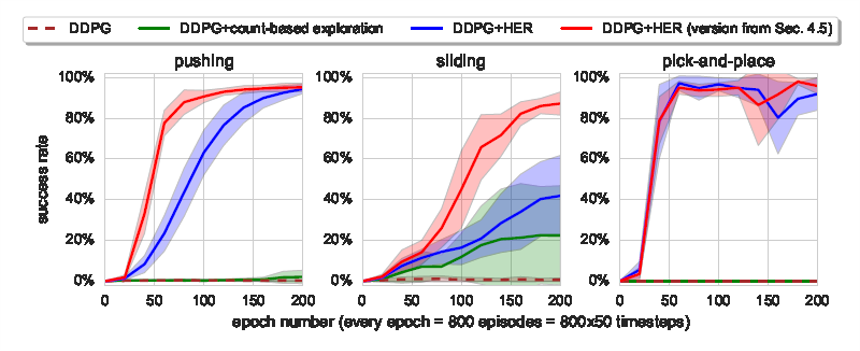
\includegraphics[width=0.9\columnwidth]{img/HER_robotic_experiments.png}
\caption{Learning curves for multi-goal setup in case of DDPG with and without HER. DDPG with HER solves the task confirming that HER is crucial for learning from sparse, binary rewards.}
\label{fig:her_robot_experiment}
\end{figure}

In summary, HER enables RL algorithms to use sparse rewards. A limitation of HER is that it is goal-oriented. It biggest advantage is that it provides more learning signals in a sparse rewards environment. HER may be seen as a form of implicit curriculum as the goals used for replay naturally shift from ones which are simple to achieve even by a random agent to more difficult ones.

\subsection{The Option-Critic Architecture}
Temporal abstraction allows representing knowledge about courses of action that take place at different time scales. In reinforcement learning, options [\cite{sutton1999between}] provide a framework for defining such courses of action and for seamlessly learning and planning with them. Based on the policy gradient theorem [\cite{sutton2000policy}], the proposal in [\cite{bacon2017option}] derives new results which enable a gradual learning process of intra-option policies and termination functions, simultaneously with the policy over them. This approach works naturally with both linear and non-linear function approximators, under discrete or continuous state and action spaces. The option critic architecture as proposed by [\cite{bacon2017option}] is shown in Fig. \ref{fig:option_critic_arch}. 
\begin{figure}[ht]
\centering
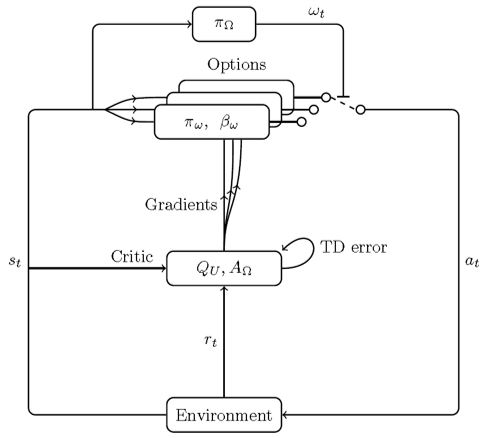
\includegraphics[width=0.9\columnwidth]{img/OptionCriticArch.png}
\caption{Diagram of the option-critic architecture. The option execution model is depicted by a \textit{switch} $\perp$ over the \textit{contacts} $\multimap$. A new option is selected according to $\pi_{\Omega}$ only when the current option terminates.}
\label{fig:option_critic_arch}
\end{figure}

The option-critic architecture works according to a \textit{call-and-return option execution model}:
\begin{enumerate}
    \item Agent picks option $\omega$ according to an inter-option policy $\pi_{\Omega}$
    \item Agent then follows an intra-option policy $\pi_{\omega}$ until termination ($\beta_{\omega}$)
    \item Repeat procedure
\end{enumerate}
The proposal in [\cite{bacon2017option}] developed a general gradient-based approach for learning simultaneously the intra-option policies and termination functions, as well as the policy over options, in order to optimize a performance objective for the task at hand.

\subsection{Learning Multi-Level Hierarchies with Hindsight}
Hierarchy has the potential to accelerate learning in sparse reward tasks because they can divide a problem into a set of short horizon sub-problems. The proposal in [\cite{levy2019learning}] introduces a framework that can learn multiple levels of policies in parallel, so the simpler sub-problems can be solved simultaneously. The framework, called \textit{hierarchical actor-critic} (HAC), has a hierarchical architecture and a method for learning multiple levels of goal-conditioned policies in parallel given sparse rewards. The number of levels in the hierarchy is a hyperparameter chosen by the user. 

The highest level policy takes as input the current state and goal state provided by the task and outputs a sub-goal state. This state is used as the goal state for the policy at the next level down. The policy at that level takes as input the current state and the goal state provided by the level above and outputs its own sub-goal state for the next level below to achieve. This process continues until the lowest level is reached. The lowest level then takes as input the current state and the goal state provided by the level above and outputs a primitive action. Further, each level has a certain number of attempts to achieve its goal state. When the level either runs out of attempts or achieves its goal state, execution at that level ceases and the level above outputs another sub-goal. Fig. \ref{fig:mutilevel_her_example} shows an example of an agent using a 3-level policy hierarchy to move through rooms to reach its target.
\begin{figure}[ht]
\centering
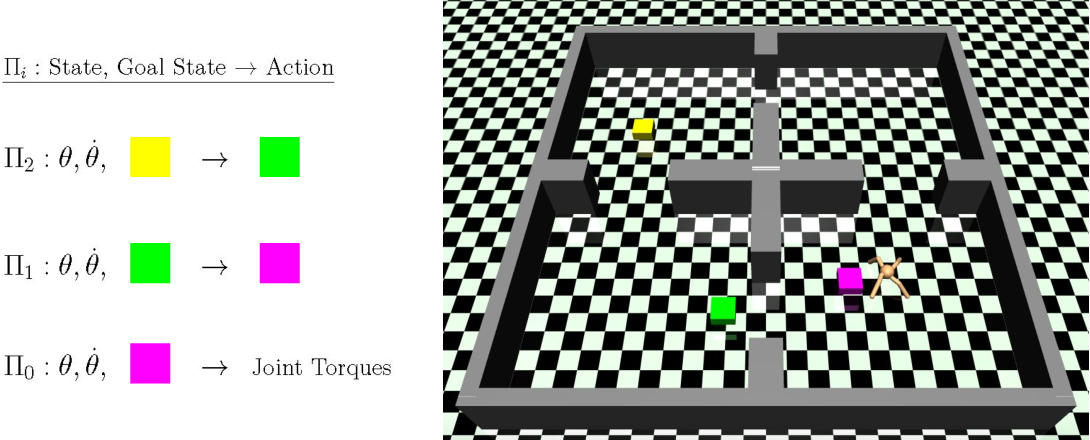
\includegraphics[width=0.9\columnwidth]{img/MultiLevelHER_example.png}
\caption{An ant agent uses a 3-level hierarchy to traverse though rooms to reach its goal, represented by the yellow cube. $\Pi_2$ uses as input the current state (joint positions $\theta$ and velocities $\dot{\theta}$) and goal state (yellow box) and outputs a sub-goal state (green box) for $\Pi_1$ to achieve. $\Pi_1$ takes in the current state and its goal state (green box) and outputs a sub-goal state (purple box) for $\Pi_0$ to achieve. $\Pi_0$ takes in the current state and goal state (purple box) and outputs a vector of joint torques.}
\label{fig:mutilevel_her_example}
\end{figure}

Experiments in [\cite{levy2019learning}] compare performance of agents using policy hierarchies with 1 (i.e., flat) and more levels with agents using Q-learning [\cite{watkins1992q}] with HER in discrete tasks and DDPG [\cite{lillicrap2015continuous}] with HER in the continuous tasks. The empirical results show that the HAC framework can benefit from additional levels of hierarchy and that multi-level agents outperform flat agents.

\section{Experiments} \label{sec:experiments}
Literature study made it clear to me that hindsight experience replay is a key method to improve training of agents in sparse reward settings. In my experiments, I implemented HER and used a Q-learning agent to measure training performance in a tabular gridworld setting. I compared the results of tabular Q-learning with HER to a baseline of tabular Q-learning without HER. From there, I tried to improve performance using new ideas. I also did experiments with HER for a robotic control task to verify whether performance of hindsight experience replay would translate to a deep learning setting.

\subsection{Tabular Q-Learning with hindsight} \label{subsec:exp_tab_her}
For this experiment, the task for the agent is to reach a position in a four-room environment in as few steps as possible. I used a small 3x3 \texttt{FourRoomsGoal-v0} environment and a larger 10x10 \texttt{FourRoomsGoalBig-v0} environment to compare how scaling up influences training efficiency. Both rooms are goal-oriented variations on the Minimalistic Gridworld Environment in [\cite{gym_minigrid}]. Fig. \ref{fig:tabular_fourroomsgoal_env} shows the \texttt{FourRoomsGoal-v0} environment.
\begin{figure}[ht]
\centering
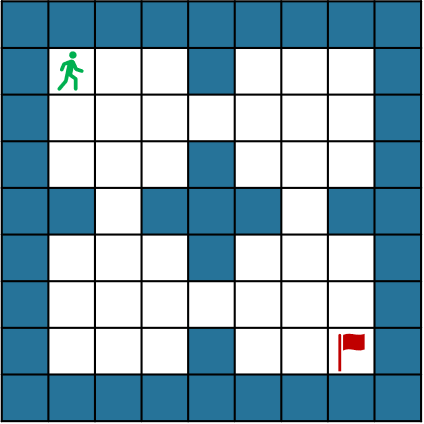
\includegraphics[width=0.5\columnwidth]{img/FourRoomsGoal-v0.png}
\caption{Goal-oriented 3x3 \texttt{FourRoomsGoal-v0} environment.}
\label{fig:tabular_fourroomsgoal_env}
\end{figure}
The setting of the experiment is:
\begin{itemize}
    \item Each training episode has random start and goal position.
    \item A sparse reward $r = 1$ is returned if goal (red flag) is reached or $r = 0$ otherwise.
\end{itemize}
In Q-learning an agent learns from every transition. During this experiment, an agent continues an episode and only stops when the goal has been reached.
In the hindsight experience replay experiments as defined in [\cite{andrychowicz2017hindsight}], good results were obtained using a \texttt{final} goal-sampling strategy where the final state in an episode is used for goal replacement in all experienced transitions of that episode. I use a slight variation on this algorithm in that I divide an episode into \textit{subtrajects} where for all transitions in a subtraject the \texttt{final} state of that subtraject is selected for goal replacement. The subtraject length is an hyperparameter then and using a grid search I tried to find the length which results in the optimal performance, i.e. the least number of steps to reach the goal state. The resulting algorithm for tabular Q-Learning with hindsight is shown in Alg. \ref{alg:qtab_her}.
\begin{algorithm}
\caption{Tabular Q-Learning with Hindsight}
\label{alg:qtab_her}
\textbf{Given}:
\begin{itemize}
    \item off-policy RL algorithm $\mathbb{A}$ (i.e. Q-learning)
    \item strategy $\mathbb{S}$ for sampling goals for replay (i.e. $\mathbb{S}(s_0, ..., s_T ) = s_T$)
    \item reward function $r: S \times A \times G \to \mathbb{R}$ (i.e. $r(s, a, g) = [f_g(s) == 1]$)
\end{itemize}
Initialize $\mathbb{A}$ (initialize q-learning agent) \\
Initialize replay buffer $R$
\begin{algorithmic}
\FOR{episode = $1, M$}
    \STATE Sample a goal $g$ and an initial state $s_0$
    \FOR{$t = 0, T-1$}
        \STATE Sample an action $a_t$ using the behavioral policy from $\mathbb{A}$: 
        \STATE \text{ }\text{ }\text{ }\text{ }$a_t \leftarrow \pi_b(s_{t}\|g)$
        \STATE Execute the action $a_t$ and observe a new state $s_{t+1}$
        \STATE $r_t := r(s_t,a_t,g)$
        \STATE Store transition $(s_t\|g, a_t, r_t, s_{t+1}\|g)$ in $R$
    \ENDFOR
    \STATE Divide episode trajectory in subtrajects of length $T_{sub}$
    \FOR{subtraject in episode}
        \FOR{$t = 0, T_{sub}-1$}
            \STATE Sample a set of additional goals for replay $G:=\mathbb{S}(\text{current subtraject})$
            \FOR{$g^{\prime} \in G$}
                \STATE $r^{\prime} := r(s_t,a_t,g^{\prime})$
                \STATE Store transition $(s_t\|g^{\prime}, a_t, r^{\prime}, s_{t+1}\|g^{\prime})$ in $R$
            \ENDFOR
        \ENDFOR
    \ENDFOR
    \FOR{$t = 1, N$}
        \STATE Sample a minibatch $B$ from the replay buffer $R$
        \STATE Perform one step of optimization using $\mathbb{A}$ and minibatch $B$
    \ENDFOR
\ENDFOR
\end{algorithmic}
\end{algorithm}

The results of tabular Q-Learning with and without hindsight experience in the 3x3 \texttt{FourRoomsGoal-v0} and the 10x10 \texttt{FourRoomsGoalBig-v0} environments are shown in Fig. \ref{fig:experiment_tabular_qlearning_her}. It's clear that Q-learning with HER outperforms Q-learning without HER because it provides more learning signals to the agent. HER has faster learning and converges faster using less optimization steps. The reason for measuring performance in function of optimization steps and not in function of the number of episodes is to have a more honest comparison between HER and non-HER experiments. HER can do more optimizations per episode because it samples mini-batches of transitions from the experience replay buffer.

\begin{figure*}[ht]
\centering
\begin{subfigure}[t]{0.45\textwidth}
\centering
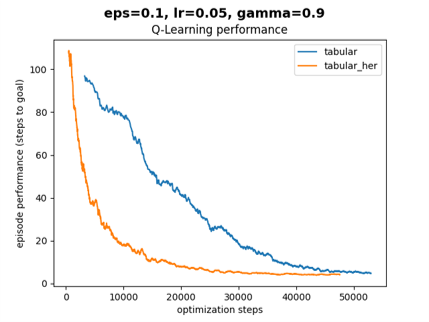
\includegraphics[width=0.9\textwidth]{img/exp_tabular_her_fourroom_small.png}
\caption{Learning curve of tabular Q-learning with and without HER for the \texttt{3x3 FourRoomsGoal-v0} environment. The results show the average performance over 10 runs of 3000 episodes each. The sub-trajectory length for Q-learning with HER equals 28 steps.}
\label{fig:experiment_fourroomsgoal_learning_performance}
\end{subfigure}
\hspace{1em}
\begin{subfigure}[t]{0.45\textwidth}
\centering
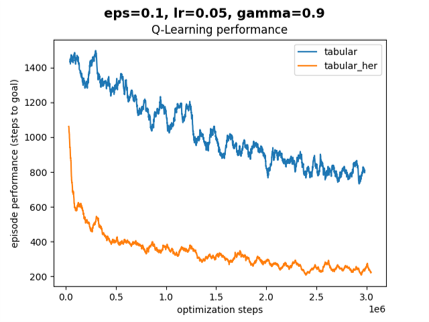
\includegraphics[width=0.9\textwidth]{img/exp_tabular_her_fourroom_big.png}
\caption{Learning curve of tabular Q-learning with and without HER for the \texttt{10x10 FourRoomsGoalBig-v0} environment. The results show the average performance over 10 runs of 20000 episodes each. The sub-trajectory length for Q-learning with HER equals 44 steps.}
\label{fig:experiment_fourroomsgoalbig_learning_performance}
\end{subfigure}
\caption{Learning curve of tabular Q-learning with and without HER for two different gridworld environments. (a) \texttt{3x3 FourRoomsGoal-v0} environment. (b) \texttt{10x10 FourRoomsGoalBig-v0} environment. The performance is measured in number of episode steps required to reach target in function of optimization steps of the Q-learning agent. Q-learning with HER has faster learning and converges faster because it provides more learning signals to the agent.}
\label{fig:experiment_tabular_qlearning_her}
\end{figure*}

The learning curves of the agent in the 3x3 \texttt{FourRoomsGoal-v0} environment (Fig. \ref{fig:experiment_fourroomsgoal_learning_performance}) shows a clear \textit{shift} to the right of both curves (HER and non-HER). This artifact is due to a smoothing algorithm which smooths results over 30 periods. This shift is less pronounced for HER because it learns faster and quickly requires less optimization steps per episode. The learning curve converges to a value of about 6 steps. This is on average the distance between the randomly assigned start and goal positions. Best case this distance is 1 step and worst case it is 12 steps.

The results for the 10x10 \texttt{FourRoomsGoalBig-v0} environment (Fig. \ref{fig:experiment_fourroomsgoalbig_learning_performance}) show an more pronounced difference in learning between HER and non-HER cases than in the smaller environment. The HER learning curve seems to converge to a value towards 200 although the curve is not yet flat after 3 million optimization steps. In the bigger environment, best case distance is 1 step and worst case distance is 40 steps. On average this would lead to an optimal value of 20 steps. An explanation to the difference between the actual curve and optimal value could be that the agent's '$\epsilon$-greedy algorithm part of the time still explores and doesn't always choose the best action. 

As mentioned before, I use a variation of the HER algorithm in which episodes are divided into subtrajects with the subtraject length used as a hyperparameter. I performed a grid search for both environments used in the experiments to find the optimal value, i.e. a subtraject length that minimizes the number of steps needed to reach the goal position in the fourroom environments. The results of this grid search are shown in Fig. \ref{fig:experiment_subtraject_gridsearch}. Although the plots are somewhat noisy due to the coarse granularity of subtraject values in the grid search, a clear trend can be noticed. For the \textit{FourRoomsGoal-v0} environment (Fig. \ref{fig:experiment_subtraject_gridsearch_small}) an optimal value of 28 was found and for the \textit{FourRoomsGoalBig-v0} environment (Fig. \ref{fig:experiment_subtraject_gridsearch_big}) this value was 44. To be sure that the values are not local minima, a more extensive grid search would be required.

\begin{figure*}[ht]
\centering
\begin{subfigure}[t]{0.45\textwidth}
\centering
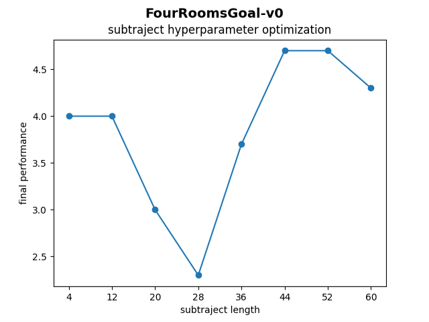
\includegraphics[width=0.9\textwidth]{img/exp_tabular_her_gridsearch_small.png}
\caption{\texttt{3x3 FourRoomsGoal-v0} performance in function of subtraject length. Optimal performance (i.e. minimum number of steps to goal) was found at subtraject length of 28 transitions.}
\label{fig:experiment_subtraject_gridsearch_small}
\end{subfigure}
\hspace{1em}
\begin{subfigure}[t]{0.45\textwidth}
\centering
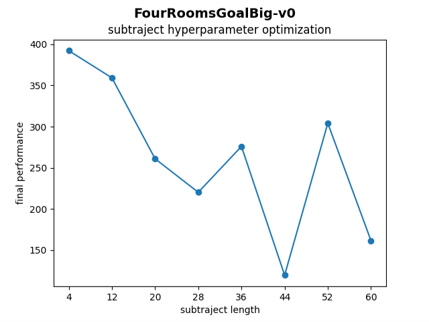
\includegraphics[width=0.9\textwidth]{img/exp_tabular_her_gridsearch_big.png}
\caption{\texttt{10x10 FourRoomsGoalBig-v0} performance in function of subtraject length. Optimal performance (i.e. minimum number of steps to goal) was found at subtraject length of 44 transitions.}
\label{fig:experiment_subtraject_gridsearch_big}
\end{subfigure}
\caption{Grid search results on the optimal subtraject length hyperparameter for the modified HER algorithm. Episodes of experience are divided into subtrajects with a fixed length. The sample strategy will sample new goals on subtraject level, rather than on traject level. The subtraject length thus determines how many different goals will be sampled and used as hindsight experience over the course of an episode.}
\label{fig:experiment_subtraject_gridsearch}
\end{figure*}

\subsection{Option Learning with Hindsight}
Knowing that we can train a Q-learning agent with HER and that it greatly improves learning over non-HER Q-learning, can we also use that agent for more complex tasks than just reaching a goal? Suppose we have an environment where we can only reach a goal if certain sub-goals are reached first. Suppose further that a meta-agent exists that can learn high-level goals (options) and a controller agent that knows how to perform low-level actions to actually reach goals. The meta-agent only knows when a final goal has been reached when it receives a sparse reward. Fig. \ref{fig:experiment_option_her_concept} shows the concept.

\begin{figure}[ht]
\centering
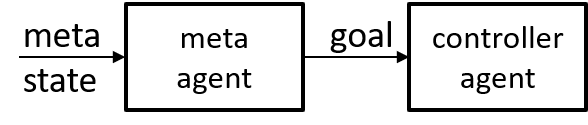
\includegraphics[width=0.9\columnwidth]{img/option_her_concept.png}
\caption{Option learning meta-agent using a controller agent to reach goals.}
\label{fig:experiment_option_her_concept}
\end{figure}

In this experiment, I created a \texttt{FourRoomsKeyDoorEnv-v0} environment with a key and a door. The environment is very similar to the \texttt{FoorRoomsGoalEnv-v0} used in \ref{subsec:exp_tab_her}, with the difference that the goal is to reach the door while having a key. The options to discover are the key and the door. I created two variants of this environment: \texttt{FourRoomsKeyDoorEnv-v0} and \texttt{FourRoomsBigKeyDoorEnv-v0} to assess training in small and big room environments. Fig. \ref{fig:experiment_option_her_keydoor_env} shows the \texttt{FourRoomsKeyDoorEnv-v0} environment.

\begin{figure}[ht]
\centering
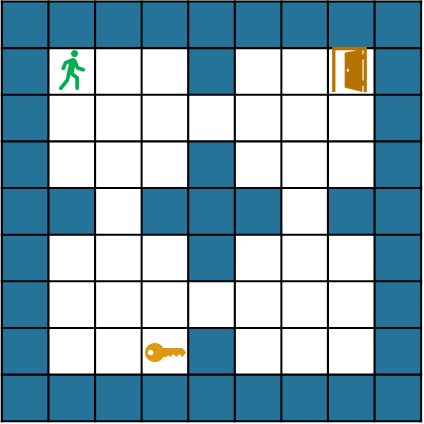
\includegraphics[width=0.5\columnwidth]{img/FourRoomsKeyDoorEnv-v0.png}
\caption{3x3 FourRoomsKeyDoorEnv-v0 environment.}
\label{fig:experiment_option_her_keydoor_env}
\end{figure}

The setting of the experiment is as follows:
\begin{description}
\item[Environment] Four rooms with key and door placed at fixed position. The observation space is described by (position, key) with key as picked-up flag. The reward function is $r = (key==1 \And position==door)$
\item[Meta-agent] Q-Learning agent. The meta-agent trains a policy to select the best goal, based on the state, i.e. key being picked up or not. The high-level goals learned are actually the options used as sub-goals for the controller agent. 
\item[Controller-agent] Q-Learning with HER agent. The controller agent is pretrained to reach goals. It's policy is trained on state described by (position, goal) and its low-level actions are basic movements \texttt{up, down, left, right}.
\end{description}

With the described setting it's straightforward to train the meta-agent as a Q-learning agent. Options are generated according to an $\epsilon$-greedy policy, while the controller agent is acting greedy according to its pretrained policy. The training performance of the meta-agent is shown in Fig. \ref{fig:exp_option_her_training_small} for the small environment.  The learning curve shows the number of options or high-level goals taken to reach the door with the key. It converges to slightly above 2 options (optimal is 2, i.e. the key and door option). The agent still explores explaining why on average the number is slightly above 2. Fig. \ref{fig:exp_option_her_training_big} shows the training performance for the big environment. Similar results are obtained.

\begin{figure*}[ht]
\centering
\begin{subfigure}[t]{0.45\textwidth}
\centering
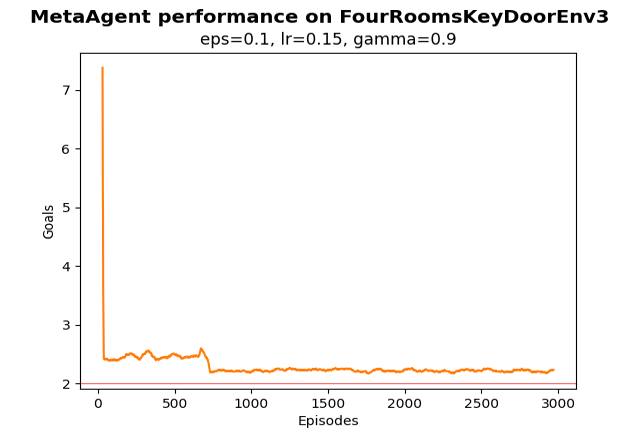
\includegraphics[width=0.9\textwidth, height=5cm]{img/exp_option_her_keydoor_small.png}
\caption{Learning curve of meta-agent option learning for the \texttt{FourRoomsKeyDoorEnv} environment.}
\label{fig:exp_option_her_training_small}
\end{subfigure}
\hspace{1em}
\begin{subfigure}[t]{0.45\textwidth}
\centering
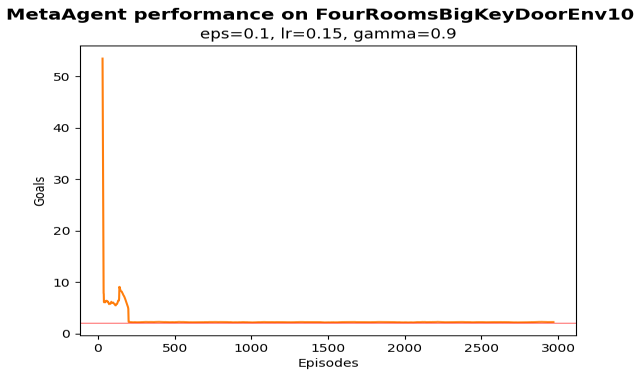
\includegraphics[width=0.9\textwidth, height=5cm]{img/exp_option_her_keydoor_big.png}
\caption{Learning curve of meta-agent option learning for the \texttt{FourRoomsBigKeyDoorEnv} environment.}
\label{fig:exp_option_her_training_big}
\end{subfigure}
\caption{Learning curve of meta-agent option learning for the (a) \texttt{FourRoomsKeyDoorEnv} environment and the (b) \texttt{FourRoomsBigKeyDoorEnv} environment. The performance is measured in number of options needed to reach target in function of episode. Results are averaged over 10 training runs of 3000 episodes each.}
\label{fig:exp_option_her_training}
\end{figure*}

As the meta-agent only has two states and as many actions as potential goals, equaling the state space for the controller agent, the agent conceptually learns in two different Qtable planes, one where the key hasn't been picked up yet, and one where the key has been picked up. These Qtable planes are shown for the \texttt{FourRoomsKeyDoorEnv} environment in Fig. \ref{fig:exp_option_her_qtable_small_key0} (key not picked up) and in Fig. \ref{fig:exp_option_her_qtable_small_key1} where the key has been picked up. Looking at the state-action values in Fig. \ref{fig:exp_option_her_qtable_small_key0}, its clear that the best option to take is goal position where the key is located in case it hasn't been picked up yet. Looking at Fig. \ref{fig:exp_option_her_qtable_small_key1}, the best option to take is the door position in case the key has been picked up. We can conclude that the meta-agent has learned the best options to perform the task optimally. Results for the bigger \texttt{FourRoomsBigKeyDoorEnv} environment are similar and the same two options are discovered.

\begin{figure*}[ht]
\centering
\begin{subfigure}[t]{0.45\textwidth}
\centering
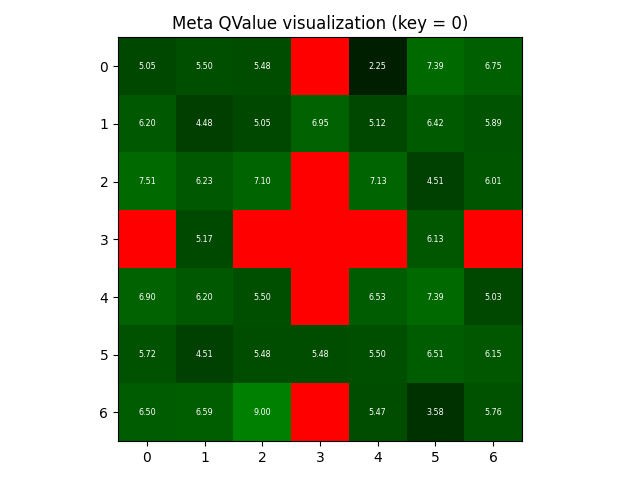
\includegraphics[width=0.9\textwidth]{img/exp_option_her_qtable_small_key0.png}
\caption{Qtable of the option learning meta-agent in state where key is not yet picked up. Best option to take is goal position where the key is located.}
\label{fig:exp_option_her_qtable_small_key0}
\end{subfigure}
\hspace{1em}
\begin{subfigure}[t]{0.45\textwidth}
\centering
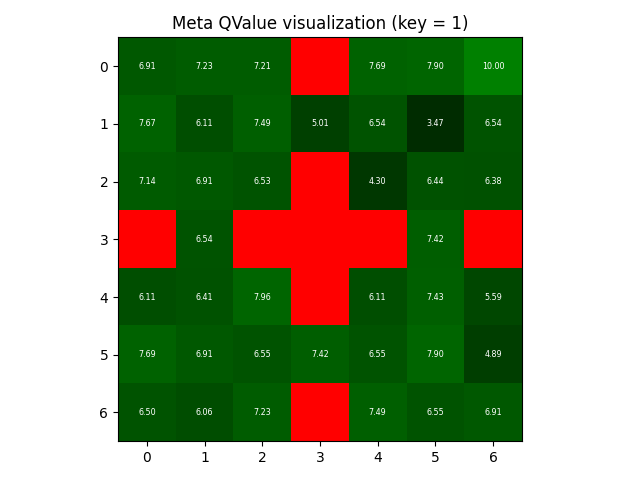
\includegraphics[width=0.9\textwidth]{img/exp_option_her_qtable_small_key1.png}
\caption{Qtable of the option learning meta-agent in state where key has been picked up. Best option to take is the door position.}
\label{fig:exp_option_her_qtable_small_key1}
\end{subfigure}
\caption{Qtable of the option learning meta-agent for the \texttt{FourRoomsKeyDoorEnv} environment. The Qtables show the state-action values after training the agent. There are only two possible states: \{key not picked up, key picked up\}. (a) Qtable in state when key has not been picked up. (b) Qtable in state when key has been picked up. Bot tables have one action with the highest state-action value, i.e. the key and door position, respectively in the state where the key hasn't been picked up yet, and the key has been picked up. These are the discovered options.}
\label{fig:exp_option_her_qtable_small}
\end{figure*}

After being trained, according to the meta-agent's Qtable values, the meta-agent should perform optimal. The results of test runs with the trained meta-agent and pretrained controller agent are shown in Tab. \ref{tab:exp_option_her_test}. For both \texttt{FourRoomsKeyDoorEnv} and \texttt{FourRoomsBigKeyDoorEnv} environments, the meta-agent only needs two high-level options to reach the door with the key and thus performs optimally. For both environments the total number of low-level actions required to complete the task is not optimal and performance in the bigger environment is worse than in the smaller one. This indicates that the pretrained controller agent could benefit from more training. The table also shows the chance that the key was picked up by accident, i.e. that a goal was chosen by the meta-agent which lead the controller agent over a path containing the key position but not landing on the key position. This would mean the key was picked up by chance, rather than following an optimal option policy. As can be seen, this was not the case during test.

\begin{table}[ht]
\centering
\begin{tabular}{|l|l|l|}
  \hline
  Metric & \texttt{Small Env} & \texttt{Big Env} \\
  \hline
  Options from start to key pick-up   & 1 & 1 \\
  Options from start to door with key & 2 & 2 \\
  Actions from start to key pick-up   & 8 & 33 \\
  Actions from start to door with key & 20 & 85 \\
  Key pick-up by chance incidence     & 0.0 & 0.0 \\
  \hline
\end{tabular}
\caption{Meta-agent and controller agent test performance statistics for the \texttt{FourRoomsKeyDoorEnv} (shortened to \texttt{Small Env} and the \texttt{FourRoomsBigKeyDoorEnv} (shortened to \texttt{Big Env}) environments. For both environments the meta-agent performs optimally and only needs one option to pick up the key and two options from start to reach the door with key. The controller agent performance is sub-optimal for both environments as it needs more actions to the door with key than the optimal path, although the agent performs worse for the big environment. The key is never picked up by chance, because the best option to reach the key position is the key position itself.}
\label{tab:exp_option_her_test}
\end{table}

As a benchmark to compare results of the option-learning agent and goal-oriented (required by HER) controller agent, I trained a baseline Q-learning agent without HER on both \texttt{FourRoomsKeyDoorEnv} and \texttt{FourRoomsBigKeyDoorEnv} environments. The results are shown in Tab. \ref{tab:exp_baseline_tabular_qlearning}. Comparing results with the option learning case, the baseline q-learning agent is better trained for the task and has superior performance in both \texttt{FourRoomsKeyDoorEnv} and \texttt{FourRoomsBigKeyDoorEnv} environments. It doesn't need to learn multiple goals like the controller agent and only learns from actual experience, where the controller agent also learned from hindsight experience which introduces bias in the learned policy. On the other hand, the baseline q-learning agent is trained specifically for this task only.

\begin{table}[ht]
\centering
\begin{tabular}{|l|l|l|}
  \hline
  Metric & \texttt{Small Env} & \texttt{Big Env} \\
  \hline
  Actions from start to key pick-up   & 8 & 19 \\
  Actions from start to door with key & 18 & 60 \\
  \hline
\end{tabular}
\caption{Baseline tabular Q-learning agent test performance statistics for the \texttt{FourRoomsKeyDoorEnv} (shortened to \texttt{Small Env} and the \texttt{FourRoomsBigKeyDoorEnv} (shortened to \texttt{Big Env}) environments. The baseline Q-learning agent performs optimally and follows a path with minimal distance from start to key pick-up position, and from there to the door for both environments.}
\label{tab:exp_baseline_tabular_qlearning}
\end{table}

To conclude, this experiment showed that we can train a Q-learning meta-agent to discover options to give to a pretrained controller agent performing the low-level actions to reach those options in order to perform more complex tasks than just reaching a single goal, and this in sparse reward setting using intrinsic motivation. It still pays off to train an agent specifically for one environment, as the baseline q-learning agent performance shows, taking into account that the learned policy will not be usable for other tasks.

\subsection{From tabular to deep learning for motor control task}
In [\cite{plappert2018multi}], a set of challenging continuous control tasks are introduced which all have binary sparse rewards and follow a multi-goal reinforcement learning framework using hindsight experience. In this experiment I tried to reproduce the results of the paper and learnt about possible new ideas for future research (see \ref{sec:future_work}). 

The setting of the experiment is as follows:
\begin{itemize}
\item \textbf{Environment}: \texttt{PandaPickAndPlace} [\cite{gallouedec2021multi}] robot environment based on PyBullet. Environment has a sparse reward: r = 1 if task is achieved, 0 otherwise.
\item \textbf{Agent}: DDPG and HER for learning. Based on implementation of OpenAI-baselines [\cite{baselines}].
\item \textbf{Task}:
    \begin{itemize}
        \item Move robot gripper to an object
        \item Pick up the object
        \item Move the object to a target place
    \end{itemize}
\end{itemize}

Experiments in [\cite{plappert2018multi}] require Mujoco robot environments, which cannot be used due to the license costs. Instead I used the Panda robot environment. Fig.\ref{fig:PandaPickAndPlace} shows \texttt{PandaPickAndPlace-v1}.
\begin{figure}[ht]
\centering
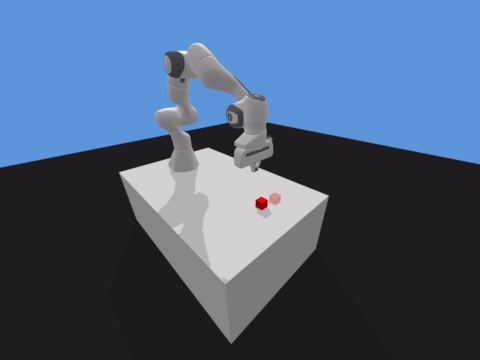
\includegraphics[width=0.6\columnwidth]{img/PandaPickAndPlace-v1.png}
\caption{\texttt{PandaPickAndPlace-v1} environment.}
\label{fig:PandaPickAndPlace}
\end{figure}

There are two versions of the \texttt{PandaPickAndPlace} environment. I initially trained an agent with version 0. Version 1 has increased friction on the object for grabbing. For both environments, I trained the agent using DDPG + HER for 3 runs with different random seeds. Each run has 50 epochs of training for 1 million of time steps in total. The success rate for training, success rate for testing and the performance test results of [\cite{plappert2018multi}] are shown in Fig. \ref{fig:exp_deep_perf}.

\begin{figure*}[ht]
\centering
\begin{subfigure}[t]{0.30\textwidth}
\centering
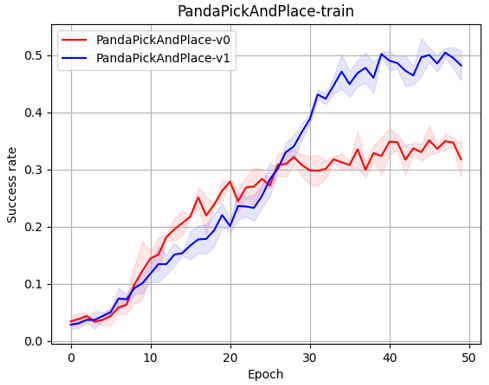
\includegraphics[width=0.9\textwidth, height=4.5cm]{img/exp_deep_train.png}
\caption{Mean training success rate (line) with standard deviation (shaded area) after each training epoch with averaged over runs with 3 different random seeds in PandaPickAndPlace-v0 and PandaPickAndPlace-v1 environment. Agent trained using DDPG+HER, 50 epochs of training with 1 million time steps in total.}
\label{fig:exp_deep_train}
\end{subfigure}
\hspace{1em}
\begin{subfigure}[t]{0.30\textwidth}
\centering
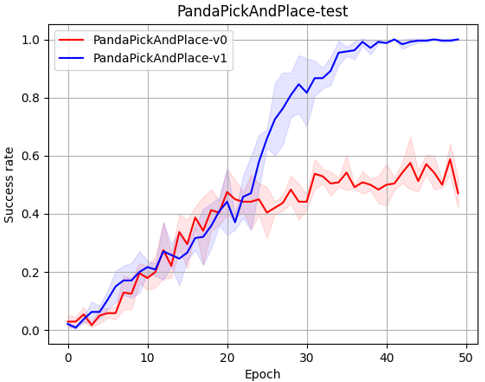
\includegraphics[width=0.9\textwidth, height=4.5cm]{img/exp_deep_test.png}
\caption{Mean test success rate (line) with standard deviation (shaded area) after each training epoch averaged over runs with 3 different random seeds in PandaPickAndPlace-v0 and PandaPickAndPlace-v1 environment.}
\label{fig:exp_deep_test}
\end{subfigure}
\hspace{1em}
\begin{subfigure}[t]{0.30\textwidth}
\centering
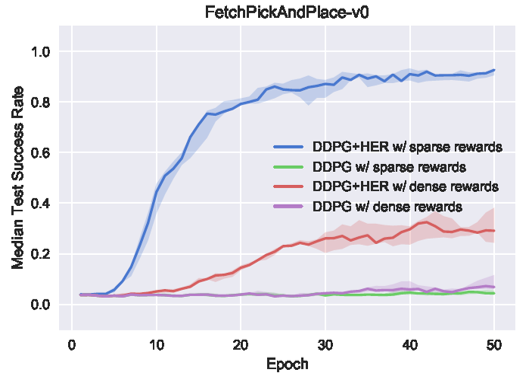
\includegraphics[width=0.9\textwidth, height=4.5cm]{img/exp_deep_test_plappert.png}
\caption{Median test success rate (line) with interquartile change (shaded area) after each training epoch averaged over runs with 5 different random seeds in FetchPickAndPlace environment ([\cite{plappert2018multi}]).}
\label{fig:exp_deep_test_plappert}
\end{subfigure}
\caption{Deep learning performance for a fetch-pick-and-place robotic control task. (a) Training success rate in PandaPickAndPlace. (b) Testing success rate in PandaPickAndPlace. After 50 training epochs, test success rate is successful half of the time for version 0 of the environment, where for version 1, the task of picking and placing the object by the robot is performed successfully. (c) Testing success rate in FetchPickAndPlace ([\cite{plappert2018multi}]). Testing results for DDPG+HER in (c) seem to converge a bit faster than the results from (b) but after 50 epochs results of (b) are close to 100\% success rate than results of (c). Overall my test results are in line with those of DDPG+HER in [\cite{plappert2018multi}].}
\label{fig:exp_deep_perf}
\end{figure*}

The success rate for testing is shown in Fig. \ref{fig:exp_deep_test}. With version 0 of the environment, we're only successful half of the time, where for version 1, the task of picking and placing the object by the robot is performed successfully after about 50 epochs of training. The results from [\cite{plappert2018multi}] are shown in Fig. \ref{fig:exp_deep_test_plappert} and seem to converge a bit faster than my own results but equally converge to nearly $100\%$ success rate after 50 episodes of training.

The results of my experiments show that we can apply the ideas from a discrete tabular Q-learning setting to a more complex, continuous deep learning setting for motor control task, In this experiment I reproduced the results of the paper [\cite{plappert2018multi}]. 

\section{Future work} \label{sec:future_work}
By assuming that experienced actions lead to successful hindsight goals, the hindsight experience replay technique ([\cite{andrychowicz2017hindsight}]) introduces bias in the learned policy. Compare a real experience tuple $(s_t\|g, a_t, r_t, s_{t+1}\|g)$ with actual goal $g$ to the artificially constructed hindsight experience tuple $(s_t\|g^{\prime}, a_t, r^{\prime}, s_{t+1}\|g^{\prime})$ with $g^{\prime}$ as hindsight goal. This conversion of a real experience to its corresponding hindsight experience makes the unjustified assumption that given different
inputs $s_t\|g$ and $s_t\|g^{\prime}$, the policy returns the same action $a_t$. This assumption overestimates the probability assigned by the policy to $a_t$, given the input $s_t\|g^{\prime}$, introducing uncertainty along the hindsight episode.

ARCHER ([\cite{lanka2018archer}]) compensates for this bias by utilizing more aggressive hindsight rewards, so that a large positive reward given to a successful hindsight transition
greatly increases the Q-value of the hindsight state-action pair, which indirectly drives an aggressive policy update towards choosing this maximizing action for the given hindsight
state.

Both HER and ARCHER do not take into account variable importance of hindsight experience at different stages of training. [\cite{vecchietti2020sampling}] proposes a sampling rate decay strategy that decreases the number of hindsight experiences as training proceeds. Hindsight experience is more important at the beginning of the training process. In this way, the action values of hindsight experiences are maximized, even with overestimated transition probabilities. As training proceeds, the rate of hindsight experience is decreased, while the rate of real experience is increased. The presence of unsuccessful real experience is also important to ensure generalization of the policy over the entire state–action space. At the end of the training, the rate of real experience is significantly higher when compared with HER and ARCHER, alleviating the bias problem as well as improving learning efficiency.

A downside of the proposed method is that a time-consuming grid search is needed to find the best values of hyperparameters which determine the decaying amount of hindsight experience used during learning and act as an adaptive learning rate.

The learning rate is the most important hyperparameter to tune for training deep neural networks. [\cite{smith2017cyclical}] describes a method for setting a cyclical learning rate, which practically eliminates the need to experimentally find the best learning rate values. The method lets the learning rate cyclically vary between reasonable boundaries. It is demonstrated that training with cyclical learning rates improves classification accuracy without the need to tune and often in fewer iterations. The paper discusses a number of cyclical learning rate (CLR) policies:
\begin{itemize}
    \item \texttt{triangular}: Linearly increasing/decreasing learning rate between minimum and maximum bounds, illustrated in Fig. \ref{fig:research_clr}.
    \item \texttt{triangular2}: The same as triangular, but with decreasing learning rate difference at each cycle.
    \item \texttt{exp\_range}: The learning rate varies between minimum and maximum boundaries and each boundary value declines by an exponential factor.
\end{itemize}
\begin{figure}[ht]
\centering
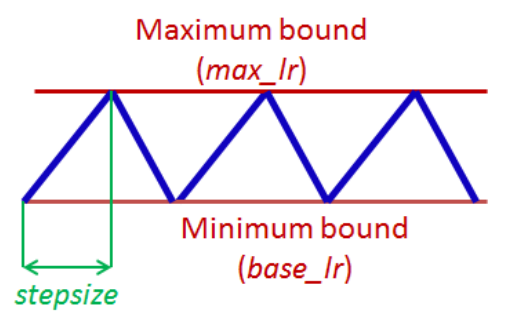
\includegraphics[width=0.7\columnwidth]{img/CLR.png}
\caption{Triangular learning rate policy. The blue lines represent learning rate values changing between bounds. The input parameter stepsize is the number of iterations in half a cycle.}
\label{fig:research_clr}
\end{figure}

Given the good results of hindsight experience sampling rate decay [\cite{vecchietti2020sampling}], and demonstrated improvements of using a cyclical learning rate (CLR) technique in classification problems [\cite{smith2017cyclical}], it is worthwhile investigating how CLR concepts can be applied in a HER sample rate decay strategy and how it could improve training efficiency. Applying those concepts would translate into varying the HER sampling rate between minimum and maximum boundaries and have each boundary decline by some exponential factor. It is also worthwhile to research what functional forms (e.g. triangular, parabolic, sinusoidal) of sampling rate offer better results.

\section{Conclusion} \label{sec:conclusion}
I presented a classification of research on intrinsic motivation and identified hindsight experience replay (HER) as novel technique to increase learning signals in sparse reward environments and as branch for further study. I carried out experiments using Q-learning agent in tabular environments and DDPG agent for robotic control tasks to train them with both actual and hindsight experience. I empirically demonstrated that HER improves sample-efficiency and training performance and that agents trained with HER can be used as controller to discover options in for a different task. I proposed potential future work to explore and improve Intrinsic Motivation using hindsight experience in Reinforcement Learning.

\section*{Acknowledgements}
I would like to thank Louis Bagot and Kevin Mets for helpful feedback and insights during the project and Louis in particular for valuable feedback on the first version of the report.

\newpage
\printbibliography
\end{document}